\chapter{OFDM}

To overcome the limitations imposed by the complexity of the equalizer in the receiver due to high data rate transmission in single carrier modulations, a multi-carrier transmission scheme approach can be adopted. In a multi-carrier transmission scheme, as the Frequency Division Multiplexing (FDM), a high data rate stream or wideband signal is divided into several low rate or narrowband parallel streams, each one called of sub-carriers, this allows the approximation of a frequency selective wideband channel by multiple non-frequency selective narrowband channels, thus reducing the complexity of the equalizer to a single tap-equalizer per sub-carrier. The basic structure of a multicarrier communication scheme is as shown in figure \ref{fig:multicarrier_diagram}, which shows that parallel symbols $x_{i}$ are transmitted in parallel subcarriers $f_{i}$ each one with a different frequency $f_{k}$. At the receiver a decoder, a filter and a oscillator is needed for every parallel subcarrier. Although the equalizer complexity in multicarrier systems is simpler than of the single carrier, its hardware implementation is more complex. The spectrum of a FDM based system with five carriers is shown in figure \ref{fig:multicarrier_fdm_spectrum}. 


\begin{figure}[hbt]
  \centering
    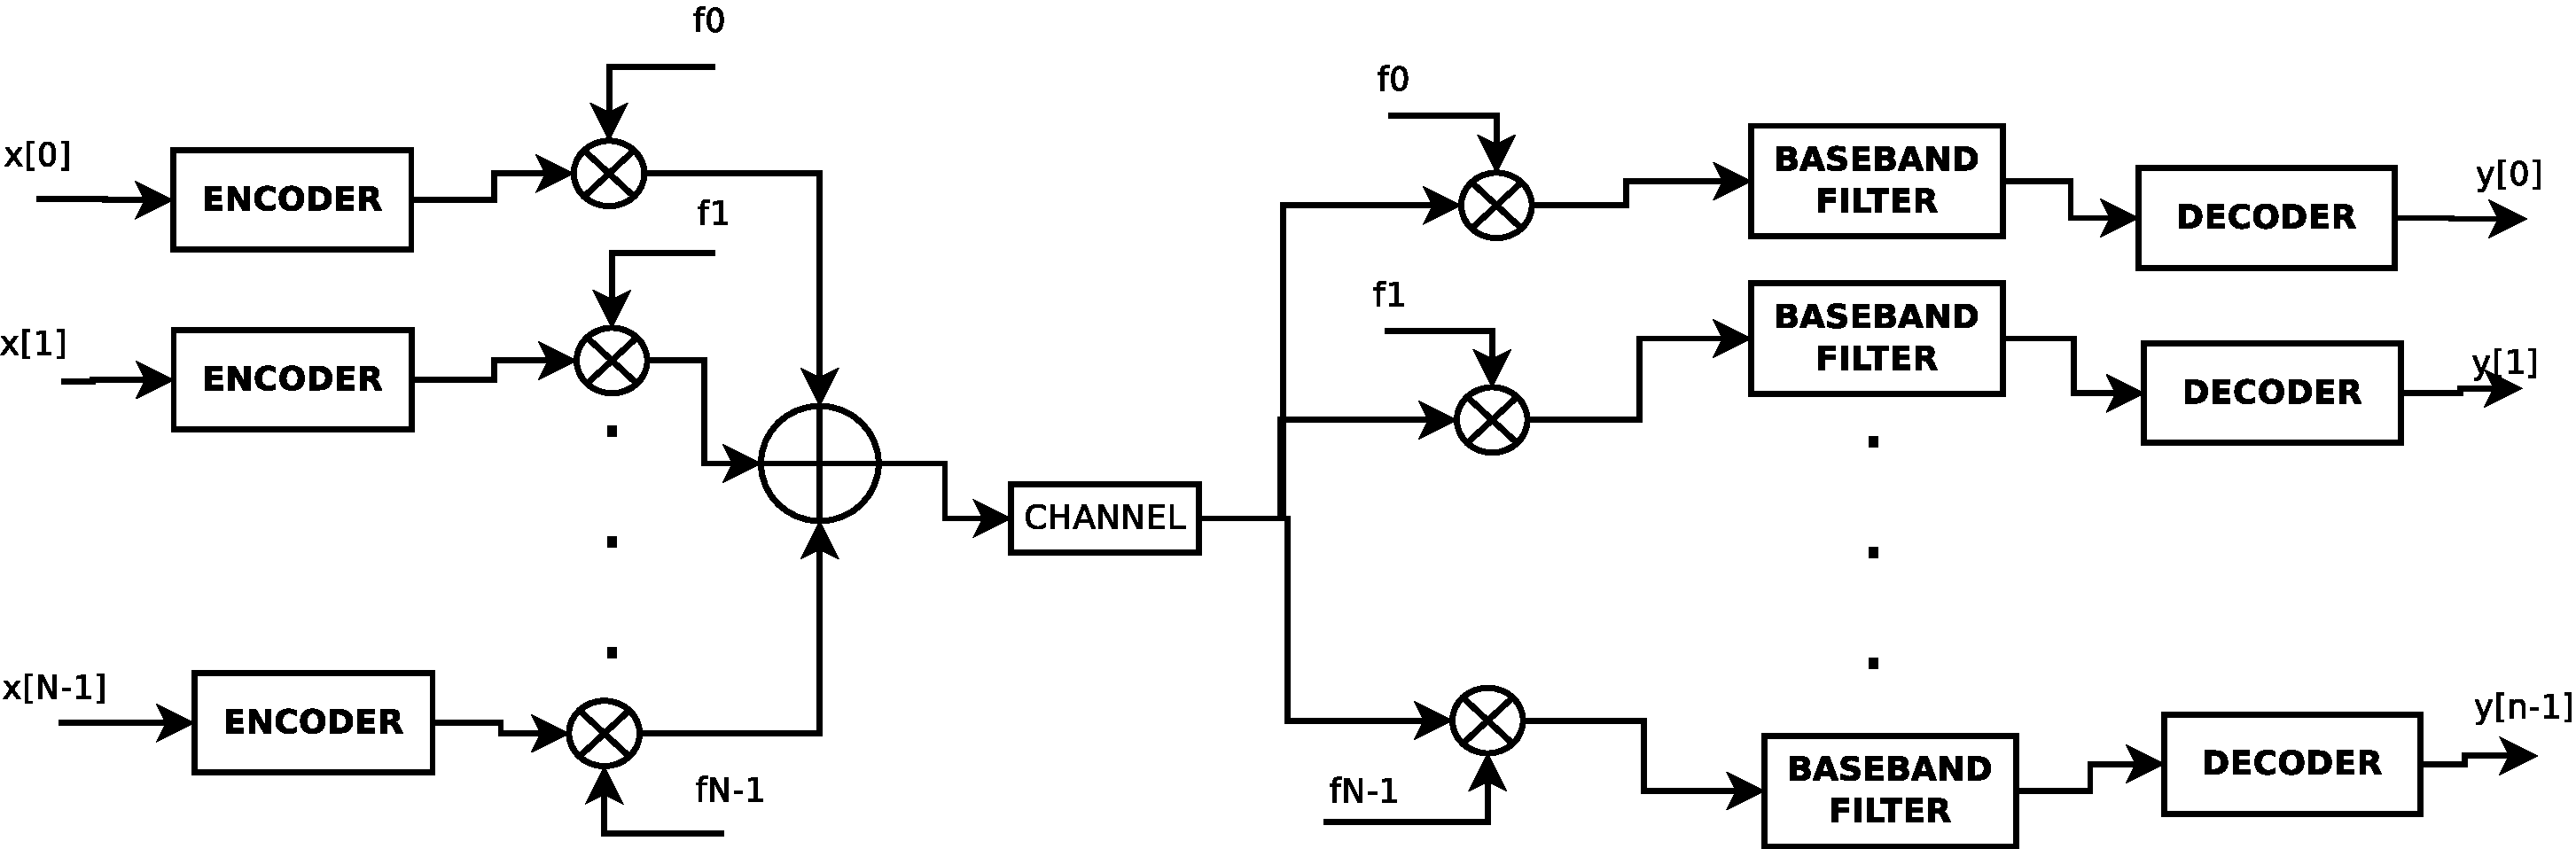
\includegraphics[width=0.9\textwidth]
      {./figures/multicarrier_diagram}
%     \rule{35em}{0.5pt}
  \caption{Multicarrier scheme basic structure}
  \label{fig:multicarrier_diagram}
\end{figure}

 
 \begin{figure}[hbt]
  \centering
    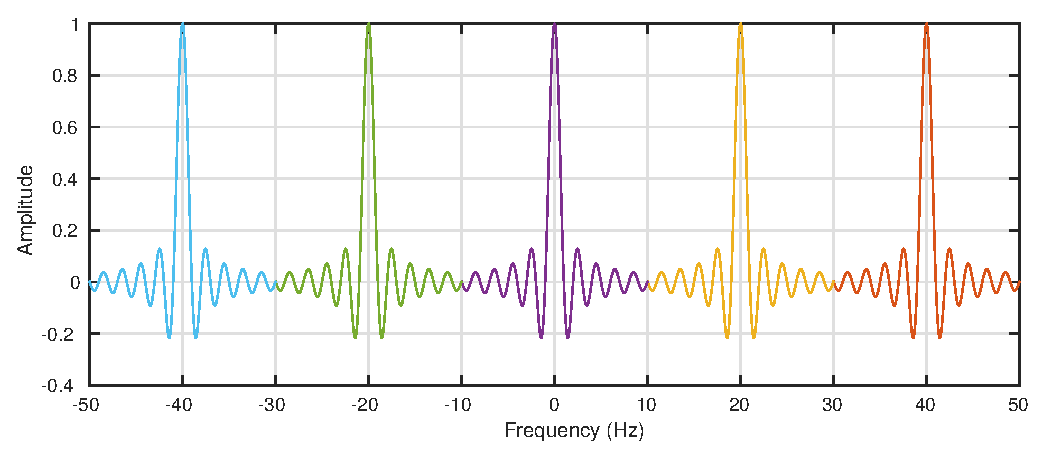
\includegraphics[width=0.9\textwidth]
      {./figures/spectrum_example_fdm}
%     \rule{35em}{0.5pt}
  \caption{Spectrum of a Multicarrier communication scheme}
  \label{fig:multicarrier_fdm_spectrum}
\end{figure}


Another type of multicarrier system that has some advantages over the multicarrier systems shown is called  Orthogonal Frequency Division Multiplexing (\ac{ofdm}). In OFDM, carriers are orthogonal among them, which saves bandwidth since its spectrum overlap.  Figure \ref{fig:multicarrier_ofdm_spectrum} shows the frequency spectrum for an OFDM system with five carriers, it can be seen that the OFDM spectrum uses much less bandwidth when compared with the multicarrier approach shown before. Another advantage of OFDM resides in its implementations. OFDM modems can be realized by means of the Inverse Discrete Fourier Transform \ac{idft} and Discrete Fourier Transforms \ac{dft}, which in turn can be efficiently implemented by the Fast Fourier Transform \ac{fft} making OFDM systems implementation less-complex than that of the multicarrier shown before. Figure \ref{fig:multicarrier_ofdm_diagram} shows the structure of an OFDM modem. Instead of the N filters, decoders and oscillators for every carrier in the parallel communication scheme, only an FFT of N points is used to perform the task. Following, OFDM modulation/demodulation process is described:


\begin{figure}[hbt]
  \centering
    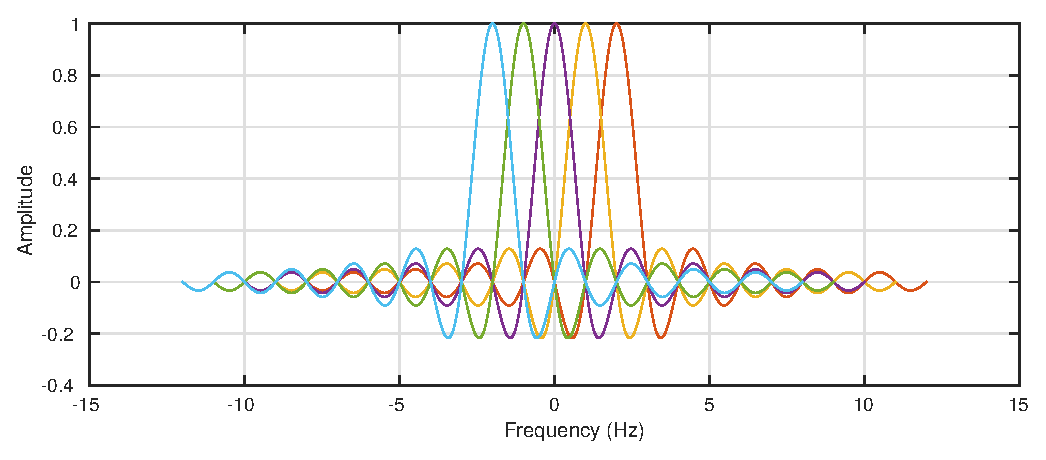
\includegraphics[width=0.9\textwidth]
      {./figures/spectrum_example_ofdm}
%     \rule{35em}{0.5pt}
  \caption{Spectrum of an OFDM communication scheme}
  \label{fig:multicarrier_ofdm_spectrum}
\end{figure}

 
\begin{figure}[hbt]
  \centering
    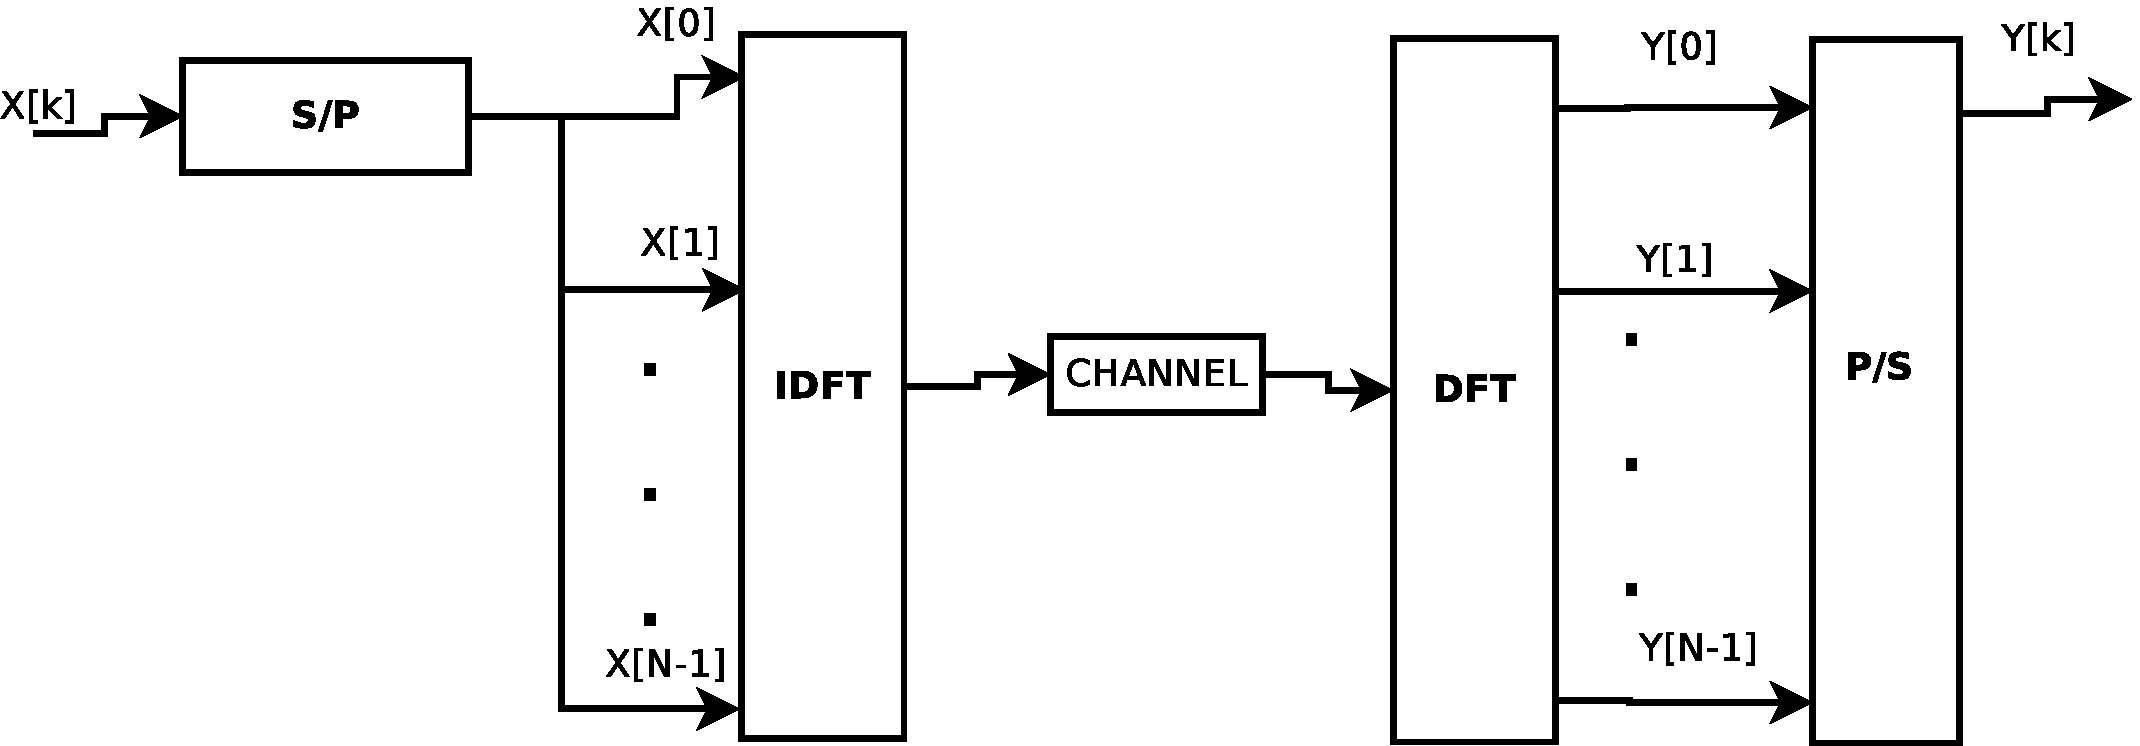
\includegraphics[width=0.9\textwidth]
      {./figures/multicarrier_diagram_ofdm}
%     \rule{35em}{0.5pt}
  \caption{OFDM basic structure}
  \label{fig:multicarrier_ofdm_diagram}
\end{figure}


 
 
%  The baseband OFDM symbol, in time domain, at the transmitter end, can be expressed as in Eq.\ref{eq:fft_out}, which 
% represents the N-point IFFT of the frequency domain signal, $S_{p}(k)$.
% %%%

% \begin{equation} 
%      x_{p}(n) = \frac{1}{N}\sum\limits_{k=0}^{N-1} S_{p}(k)e^{\frac{j2{\pi}nk}{N}}, \qquad n = 0,1,...,N-1
%     \label{eq:fft_out}
% \end{equation}

%  The transmitted frequency-domain symbol, $S_{p}(k)$, 
% can be recovered by Eq. \ref{eq:fft_out2}, which is the N-point FFT of the transmitted symbol $x_{p}(n)$.
% %%%

% \begin{equation} 
%      S_{p}(k) = \sum\limits_{n=0}^{N-1} x_{p}(n)e^{\frac{-j2{\pi}nk}{N}}, \qquad k = 0,1,...,N-1
%     \label{eq:fft_out2}
% \end{equation}
 
 

%The Orthogonal Frequency Division Multiplexing (OFDM)  technique divides a high data rate stream into several low rate parallel streams, this is achieved by sending every low data rate stream through narrow band flat fading subchannels or subcarriers,  attaining more robustness against ISI since symbol duration is reduced.    


%dividing the frequency selective fading channel into smaller narrow band sub channels, then every low data rate stream is sent in parallel through the subchannels attaining more robustness against Inter symbol Interference (ISI) since symbol duration  %By dividing the available This adds robustness against multi path fading channel, as well as a simpler equalization. 

An OFDM symbol can be described by:


\begin{equation}
S_l(t) = \sum_{k = 0}^{N-1}X_l(k)e^{j2\pi f_kt}, \quad 0 < t < T_s
\label{eq:symbol_ofdm}
\end{equation}

Where, $X_l(k)$ represents the $l_{th}$ OFDM symbol at the $k_{th}$ sub-carrier within an OFDM symbol of duration $T_{s}$ and $\Delta_f$ as the subchannel or subcarrier space for $k = 0, 1, \dotsc, N - 1$. In the OFDM transmission, the information data bits are first mapped into a single carrier symbol, e.g. QAM or QPSK symbols,  and then converted into N parallel streams. This parallel stream of symbols is then carried out by N orthogonal sub-carriers signals whose spectra overlaps in frequency domain achieving high bandwidth efficiency \cite{cho2010mimo}. 

Since it is assumed that the OFDM carriers are orthogonal, two sub-carriers, $\phi_{k}$ and $\phi_{i}$ must met the following condition:

% \begin{align*}
%  \frac{1}{T_s} \int_{0}^{T_s} e^{j2\pi f_kt} e^{-j2\pi f_it} =  \frac{1}{T_s} \int_{0}^{T_s} e^{j2\pi (f_k - f_i)t}   \\
%   =  \frac{1}{T_s} \int_{0}^{T_s} e^{j2\pi (f_k - f_i)t}   \\
%   =  \frac{1}{T_s} \int_{0}^{T_s} e^{j2\pi (f_k - f_i)t}   
% \end{align*}

\begin{align}
  \frac{1}{T_s} \int_{0}^{T_s} \phi_{k}(t) \phi_{i}^{*}(t) dt & = \frac{1}{T_s} \int_{0}^{T_s} e^{j2\pi f_kt} e^{-j2\pi f_it} dt   \nonumber \\   
  & =  \frac{1}{T_s} \int_{0}^{T_s} e^{j2\pi (f_k - f_i)t} dt    \nonumber \\
  & =  \frac{1}{T_s} \int_{0}^{T_s} e^{j2\pi (k-i)\Delta_f}  dt  \nonumber \\
  & =   \delta[k-i].
\label{eq:ortho_signals}
\end{align}

% \begin{eqnarray}
%  \frac{1}{T_s} \int_{0}^{T_s} e^{j2\pi f_kt} e^{-j2\pi f_it} dt =  \frac{1}{T_s} \int_{0}^{T_s} e^{j2\pi (f_k - f_i)t} dt  \\
%   =  \frac{1}{T_s} \int_{0}^{T_s} e^{j2\pi (k-i)\Delta_f}  dt \nonumber \\
%   =   \delta[k-i] \nonumber 
%   \label{ortho_signals}
% \end{eqnarray}


The function $\delta[k-i]$ is defined as:


\begin{equation}
\delta[n] = 
\begin{cases}
1, \quad if \quad n = 0\\
 \\
0, \quad otherwise
\end{cases}
\end{equation}

At the receiver the signal can be recovered using the orthogonality property of equation~\ref{eq:ortho_signals}, as shown in equation~\ref{eq:demod_ofdm}, where $S_r(t)$ is the received signal and $S_l(t)$ the sent signal: 

\begin{align}
S_r(t) & = \frac{1}{T_s} \int_{0}^{k = 0} S_l(t)e^{-j2\pi f_kt} dt \\
 & = \frac{1}{T_s} \int_{0}^{k = 0} \sum_{i = 0}^{N-1}X_le^{j2\pi f_it}e^{-j2\pi f_kt} dt \nonumber \\ 
 & = \sum_{i = 0}^{N-1}X_l\delta[i - k] \nonumber \\ 
 & = X_l . \nonumber \\ 
\label{eq:demod_ofdm}
\end{align}


Sampling the OFDM symbol at intervals of $\frac{T_s}{N}$ yields:


\begin{equation}
S_l(n) = \sum_{k = 0}^{N-1}X_le^{j2\pi f_k n\frac{T_s}{N}  } .
\label{eq:symbol_ofdm_discrete}
\end{equation}

If $f_0 = 0$ then, $f_kT_s = k$ 

\begin{equation}
S_l(n) = \sum_{k = 0}^{N-1}X_le^{j2\pi n\frac{k}{N}  } .
\label{eq:symbol_ofdm_idft}
\end{equation}

Equation \ref{eq:symbol_ofdm_idft} is known as the IDFT of $X_l$. Thus, the OFDM modulation/demodulation can be implemented as a IDFT/DFT pair as shown in figure \ref{fig:multicarrier_ofdm_diagram}. As mentioned before, this simplifies the OFDM transmitter/receiver complexity since no filters or encoders/decoders are used in the modulation/demodulation process. Instead IDFT/DFT are used, which that can be computed efficiently by the FFT algorithm. 

OFDM signals often show bandwidth spillage or leakage, which causes adjacent channel interference (\ac{aci}), since sub-carriers are time limited and no band limited. To avoid \ac{aci}, null carriers are added at the edges of the OFDM symbol. Null carriers at the adjacencies of the OFDM symbol also protect the OFDM signal from leakage from other adjacent systems. In general, another null sub-carrier is the Direct Current (\ac{dc}) sub-carrier, this null sub-carrier corresponds to the zero frequency sub-carrier. If the signal is not modulated, this null subcarrier is added to avoid a DC in the OFDM symbol. This helps in the Digital to Analog and Analog to digital conversion~\cite{nuaymi2007wimax}. Figure \ref{fig:ofdm_symbol_freq} shows an OFDM symbol with 64 sub-carriers in frequency domain, DC, guard band and data carriers are shown in the figure. 

\begin{figure}[hbt]
  \centering
    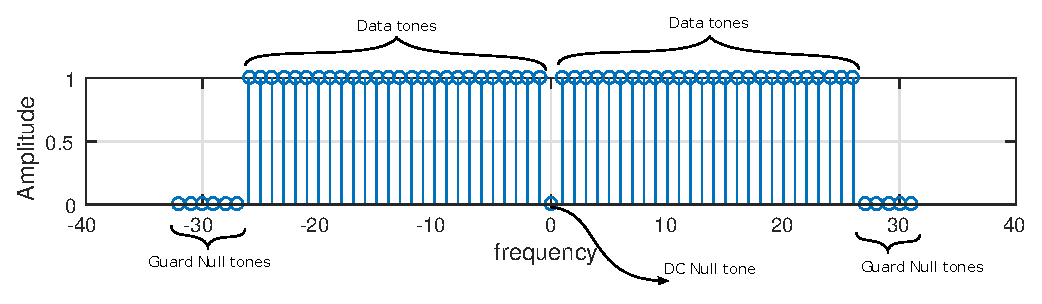
\includegraphics[width=0.9\textwidth]
      {./figures/ofdm_symbol_freq}
%     \rule{35em}{0.5pt}
  \caption{OFDM symbol with 64 sub-carriers in frequency domain}
  \label{fig:ofdm_symbol_freq}
\end{figure}

Another modification that is performed over the OFDM symbol in time domain, is that a copy of the last $G$ samples of the OFDM symbol is prepended to itself, to prevent Inter Symbol Interference (\ac{isi}). The prepended part is known as the Cyclic Prefix (\ac{cp}). ISI is originated by the multi-path fading channel, that causes that a delayed, attenuated and phase shifted copy of the previously sent signal to interfere with the arriving signal. The receiver signal can be modeled by in time domain as:

%and as in equation~\ref{eq:symbol_rx_chnnl_noise} in frequency domain.


%arrives at the receiver, interfering with the arriving signal. 


\begin{eqnarray}
y(n) = {x(n)*h(n)} + z(n) = \sum_{m=0}^{\infty}{x(m)h(n-m)} + z(n).
\label{eq:symbol_ofdm_channel}
\end{eqnarray}

\noindent where, $y(n)$ is the received signal, $x(n)$ the sent signal, and $h(n)$ the impulse response of the multi-path fading channel. The effect of multi-path channel is illustrated in figure~\ref{fig:isi_symbols}. There we see the delayed sent signal overlapping with the current received symbol and interfering with the next symbol at the receiver. The received signal in frequency domain is represented by equation~\ref{eq:symbol_rx_chnnl_noise_freq}.  

\begin{align}
Y(k) & = \sum\limits_{n= 0}^{N-1} [ {x(n)*h(n)} + z(n) ] e^{\frac{-j2{\pi}kn}{N}} \\ 
& = \sum\limits_{n= 0}^{N-1} [ \sum_{m=0}^{N-1}{x(n)h(n-m)} + z(n) ] e^{\frac{-j2{\pi}kn}{N}} \nonumber \\ 
&  = \sum\limits_{m= 0}^{N-1} \sum_{n=0}^{N-1}{x(m)h(n-m)} e^{\frac{-j2{\pi}kn}{N}} + Z(k) \nonumber \\
&  = \sum\limits_{m= 0}^{N-1} x(m) \underbrace{\sum_{n=0}^{N-1}{h(n-m)} e^{\frac{-j2{\pi}kn}{N}}}_{DFT circular shift property} + Z(k) \label{eq:circ_conv_dft_circ_shift} \\
&  = \sum\limits_{m= 0}^{N-1} {x(m)H(k)}e^{\frac{-j2{\pi}km}{N}} + Z(k) \nonumber \\
&  = H(k) \sum\limits_{m= 0}^{N-1} {x(m)}e^{\frac{-j2{\pi}km}{N}} + Z(k) \nonumber \\
&  = X(k)H(k) + Z(k) 
\label{eq:symbol_rx_chnnl_noise_freq}
\end{align}


According to equation~\ref{eq:symbol_rx_chnnl_noise_freq}, the channel compensation can be accomplished by simply dividing the received symbol in frequency domain by the channel response, i.e. $X(k) = Y(k)/H(k)$, which represents a one tap equalizer. Also $Y(k)=X(k)H(k)$ is true only when $ y(n) = x(n) \circledast y(n)$, where $\circledast$ denotes circular convolution. This makes possible to apply the DFT circular shift property in equation~\ref{eq:circ_conv_dft_circ_shift}, the circular convolution holds true only when the CP is prepended to the OFDM symbol \cite{cho2010mimo}.

%According to equation~\ref{eq:symbol_rx_chnnl_noise_freq} result, the channel compensation can be accomplished by simply dividing the received symbol in frequency domain by the channel response, that is $X(k) = Y(k)/H(k)$, which represents a one tap equalizer. Also $Y(k)=X(k)H(k)$ is true only when $ y(n) = x(n) \circledast y(n)$, where $\circledast$ denotes circular convolution (Convolution theorem), this makes possible to apply the DFT circular shift property in equation~\ref{eq:circ_conv_dft_circ_shift}, this relationship holds true only when the CP is prepended to the OFDM symbol \cite{cho2010mimo}.


\begin{figure}[hbt]
  \centering
    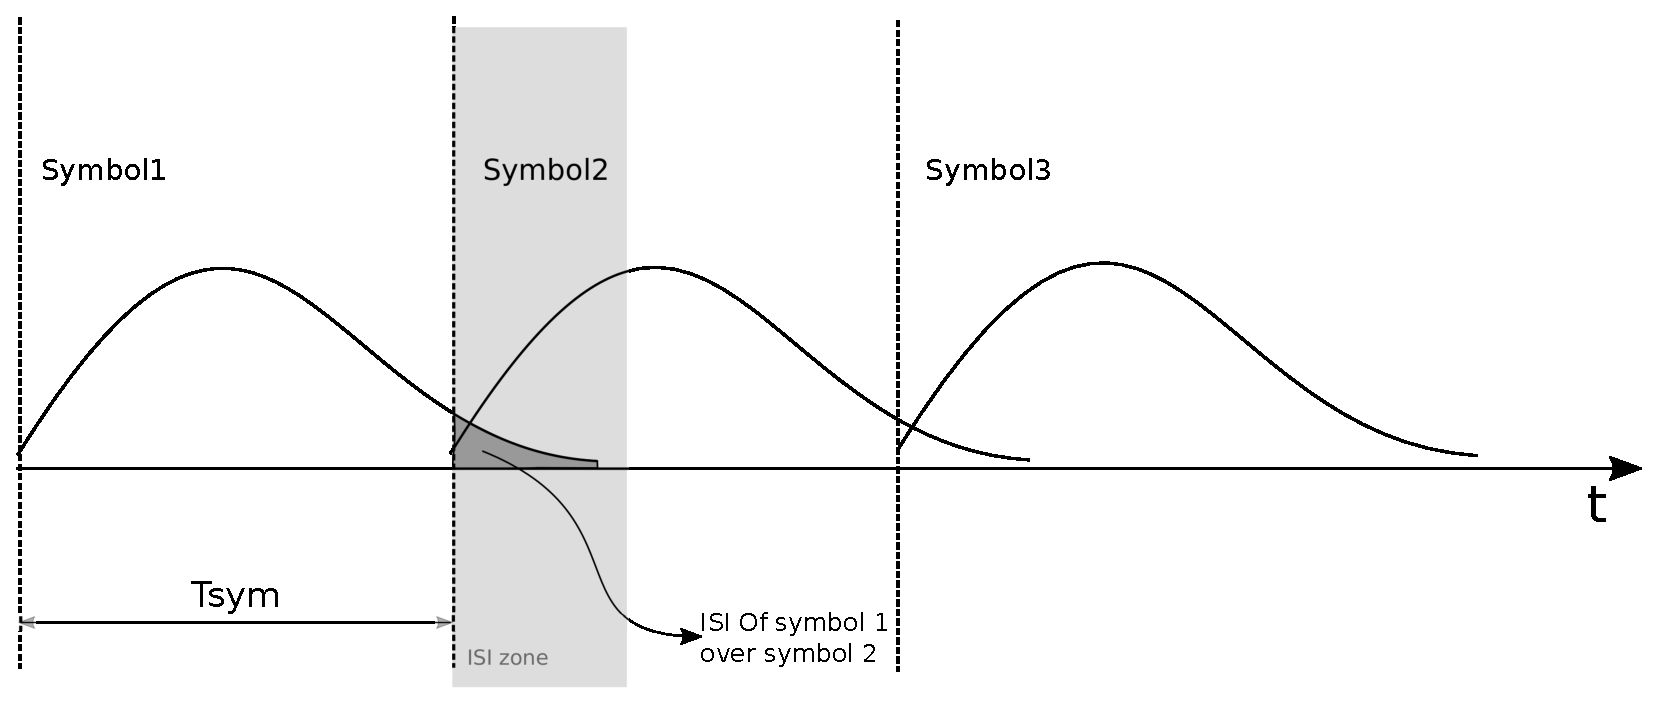
\includegraphics[width=0.8\textwidth]
      {./figures/isi_fig}
%     \rule{35em}{0.5pt}
  \caption{ISI effect over adjacent symbols}
  \label{fig:isi_symbols}
\end{figure}

 The CP appended to the beginning of the OFDM symbol in time domain safeguards the OFDM symbol from being affected by the multi-path fading channel effect over the previous transmitted symbol, as long as the channel delay is shortest than that of the duration of the CP. Figure \ref{fig:isi_symbols_cp} illustrates the effect of ISI over the OFDM symbol when the CP is added. 

\begin{figure}[hbt]
  \centering
    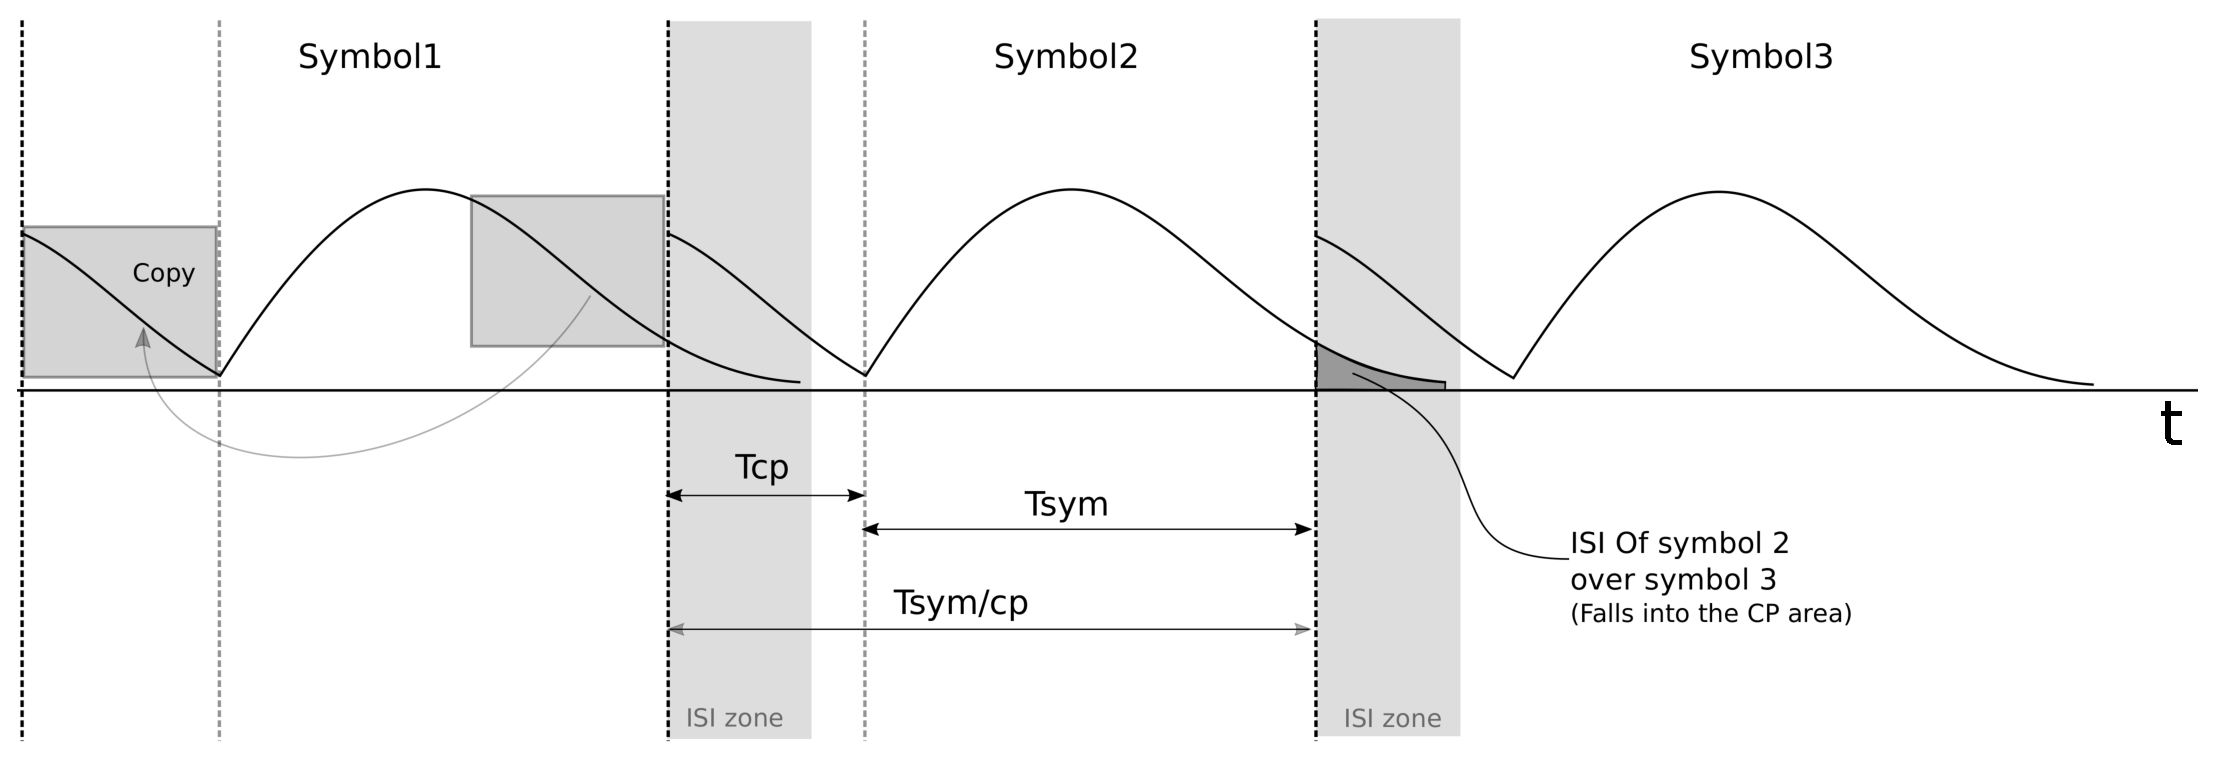
\includegraphics[width=0.9\textwidth]
      {./figures/isi_cp_2}
%     \rule{35em}{0.5pt}
  \caption{ISI effect over adjacent symbols with CP}
  \label{fig:isi_symbols_cp}
\end{figure}


\subsection{Synchronizations Errors in OFDM}

Although OFDM is widely used due to its robustness against frequency-selective fading channel as well as the reduced complexity single-tap equalizer per subcarrier \cite{chiueh2012baseband} it has large Peak to Average Ratio (PAPR)~\cite{prasad2004ofdm} and is very sensitive to the receiver synchronization errors~\cite{ber_cfo_ofdm}, such as Symbol Time Offset (\ac{sto}), i.e. finding the start of the OFDM symbol unknown at the receiver, and Carrier Frequency Offset (CFO) caused mainly by the frequency mismatch between local oscillators at the receiver and transmitter. Synchronization errors as STO and ICFO can cause Inter Symbol Interference (ISI) and Inter Carrier Interference (ICI) that hinders the proper recovery of the OFDM symbols and degrades system performance. Thus, the receiver must estimate and compensate those errors in order to properly recover the symbols. Following, the effects of those errors over the OFDM symbols are analyzed. 


\subsubsection{Carrier Frequency Offset}
\label{sec:icfo}

 
 The tolerance of local and remote oscillators causes a difference between the transmitter and receiver carrier frequency. This difference in frequencies, known as carrier frequency offset (\ac{cfo}), has some detrimental effect on sub-carriers,  hindering the symbols recovery. It can be divided into two parts regarding the sub-carrier space, a fractional frequency offset, which is a fraction of the sub-carrier spacing, and an Integer Carrier Frequency Offset (ICFO) which occurs in multiples of the sub-carriers distance.   
    
  The fractional part causes Inter Carrier Interference (\ac{ici}) due to lost of orthogonality between sub-carriers. It is typically corrected in two steps, first a coarse estimation/correction is performed followed by a fine frequency estimation/correction. On the other hand, the integer part causes a circular shift of the sub-carrier indexes in the frequency domain. It is usually estimated in frequency domain and its correction can be performed either in time or frequency domain. 

Assuming perfect symbol synchronization, i.e. zero Symbol Time Offset (the frame start is perfectly located), and without considering the impairments introduced by the channel, the transmitted symbol is frequency domain is described by equation \ref{eq:symbol_freq}, while received symbol in time domain can be described by Eq.~\ref{eq:ifft_cfo}. 
%, it is given by the IFFT of the \emph{p-th} symbol in frequency domain shifted by $\beta$.  

\begin{equation} 
     X_{p}(k) = \sum\limits_{n=0}^{N-1} x_{p}(n)e^{\frac{-j2{\pi}kn}{N}}, \qquad k = 0,1,...,N-1
    \label{eq:symbol_freq}
\end{equation}



\begin{equation} 
     y_{p}(n) = \frac{1}{N}\sum\limits_{k=0}^{N-1} X_{p}(k+\beta)e^{\frac{j2{\pi}kn}{N}}, \qquad n = 0,1,...,N-1
    \label{eq:ifft_cfo}
\end{equation}


\noindent where $\beta = \epsilon + k_{o}$ is the frequency offset, divided in $\epsilon$, the fractional frequency offset and $k_{o}$ the integer frequency offset. $X_p(k)$ the transmitted symbol in frequency domain with $k$ sub-carriers, $x_p(n)$ in time domain and $y_p(n)$ the received signal in time domain. Assuming a fractional frequency offset of zero ($\beta = k_{o}$), the term $X_{p}(k+\beta)$ can be written as in eq.~\ref{eq:ifft_symbol_shifted}

\begin{equation} 
X_{p}(k+\beta) = \sum\limits_{b=0}^{N-1} x_{p}(b)e^{\frac{-j2{\pi}(k+\beta)b}{N}}, \qquad k+\beta = 0,1,...,N-1 .
    \label{eq:ifft_symbol_shifted}
\end{equation}

% \begin{equation} 
%      r_{k} = e^{\frac{j2{\pi}n(k_{o}+\epsilon)}{N}}\sum\limits_{m=0}^{q} x_{k}h_{m} + n_{k}, 
%     \label{eq:symb_rx}
% \end{equation}
So, Eq.~\ref{eq:ifft_cfo} can be written as: %Eq.~\ref{eq:ifft_cfo_symbol_shifted}

\begin{equation} 
     y_{p}(n) = \frac{1}{N}\sum\limits_{k=0}^{N-1} \Big\{ \sum\limits_{b=0}^{N-1} x_{p}(b)e^{\frac{-j2{\pi}(k+\beta)b}{N}} \Big\} e^{\frac{j2{\pi}kn}{N}}, \qquad n = 0,1,...,N-1.
    \label{eq:ifft_cfo_symbol_shifted}
\end{equation}

\begin{equation} 
     y_{p}(n) = \frac{1}{N}\sum\limits_{b=0}^{N-1}x_{p}(b)e^{\frac{-j2{\pi}\beta b}{N}} \sum\limits_{k=0}^{N-1} e^{\frac{j2{\pi}k(n-b)}{N}} , \qquad n = 0,1,...,N-1.
    \label{eq:ifft_cfo_symbol_shifted_2sum}
\end{equation}


%%%%%%%%%%%%OJO LEER Y REDACTAR DE NUEVO%%%%%%%%%%%%%%%%%%%%%%%%%%%%%%%%%%%%%%%%%%%%%%

%If the index $b = n$ then, the variable $b$ in the first summation becomes a constant, and the complex variable exponent in the second summation becomes zero, given N as the summation result. The $p^{th}$ symbol in time domain can be expresed as eq.~\ref{}

%%%%%%%%%%%%%%%%%%%%%%%%%%%%%%%%%%%%%%%%%%%%%%%%%%%%%%%%%%%%%%%%%%%%%%%%%%%%%%%%%%%%%%%

If the index $b = n$, then the $p_{th}$ symbol in time domain can be expressed as eq.~\ref{eq:ifft_cfo_symbol_shifted_time}

\begin{equation} 
     y_{p}(n) = x_{p}(n)e^{\frac{-j2{\pi}\beta n}{N}}, \qquad n = 0,1,...,N-1.
    \label{eq:ifft_cfo_symbol_shifted_time}
\end{equation}

% %where, $n_{k}$ is the noise sample, $h$ is the channel impulse response, $\epsilon$ is a
% normalized fractional carrier frequency offset and $k_{o}$ is the normalized ICFO, which is the impairment to be 
% tackled by the algorithm that will be presented in section~\ref{sec:fft_cfo_architecture}. The presence of ICFO causes an incorrect tone numbering at the FFT output,

From eq.~\ref{eq:ifft_cfo_symbol_shifted_time} can be concluded that, the received symbol has the same value than that of the transmitted symbol with its phase rotated by $-j 2 \pi  \beta n/N$. As the fractional part is equal to zero, the integer frequency offset effect over the sub-carriers in frequency domain is a shift, as shown in the illustrative example of figure \ref{fig:icfo_example}.  
 
 \begin{figure}[hbt]
  \centering
    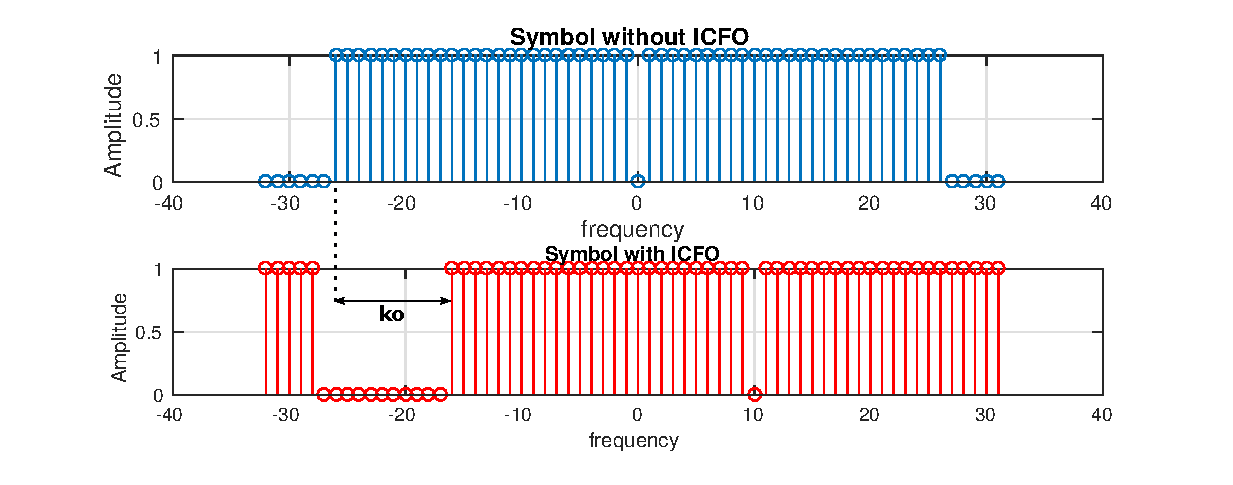
\includegraphics[width=1\textwidth]
      {./figures/icfo_shift}
%     \rule{35em}{0.5pt}
  \caption{Integer Carrier Frequency Offset of $k_{o}$ subcarriers - without error(top), with error (bottom)}
  \label{fig:icfo_example}
\end{figure}

 \subsubsection{Symbol Time Offset}
\label{sec:symbol_time_offset}

  Another impairment regarding synchronization is the symbol time synchronization error. Timing synchronization algorithms attempt to find the start of the OFDM symbol and correct what is called the STO, defined as the difference between the exact symbol start and the estimated one. The STO must be zero, so that the result of the FFT computation matches that of the transmitted symbol in frequency domain. 
  
  
  \begin{figure}[!hbt]
  \centering
    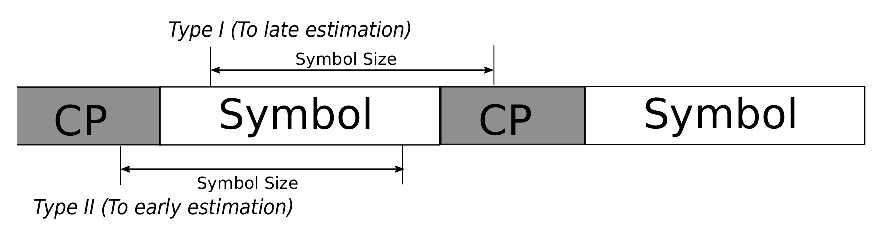
\includegraphics[width=0.8\textwidth]
      {./figures/STO_symbol}
%     \rule{35em}{0.5pt}
  \caption{STO early and late estimation}
  \label{fig:sto_estimation}
\end{figure}


 A deviation from the ideal STO can be found after the estimation process as shown in figure~\ref{fig:sto_estimation}. STO can be estimated to early or to late, regarding the ideal case in which the exact point is expected to be. A late estimation (type I, as shown in figure \ref{fig:sto_estimation}), which takes the starting point after the ideal case, generates a time windows that is shifted onto the next symbol, that is, samples from the current symbol are lost and samples from the next symbol are taken. In this case ICI is found and the orthogonality between sub-carriers is lost~\cite{cho2010mimo}. 


  The second type of offset found is the one in which the starting point is estimated to early (type II, in figure~\ref{fig:sto_estimation}), that is before the ideal starting point. In this case the first sample of the symbol falls inside the symbol CP and the last samples are lost, no samples from the next symbols are taken. In this case, the orthogonality between sub-carriers is preserved and only a phase offset proportional to the STO and the carrier index is shown in the post-FFT signal~\cite{cho2010mimo}.
  
If the STO falls inside the CP of the current symbol, and without considering the impairments introduced by the channel, the received signal can be expressed as:

\begin{equation} 
     S_{p}(k) = \sum\limits_{n=0}^{N-1} x_{p}(n+\alpha)e^{\frac{-j2{\pi}nk}{N}}, \qquad k = 0,1,...,N-1
    \label{eq:symbol_rx_sto}
\end{equation}

\noindent where the shifted symbol then can be rewritten  as:

\begin{equation} 
x_{p}(n+\alpha) = \sum\limits_{b=0}^{N-1} X_{p}(b)e^{\frac{j2{\pi}(n+\alpha)b}{N}}, \qquad b = 0,1,...,N-1
    \label{eq:fft_symbol_shifted_time}
\end{equation}

Substituting equation~\ref{eq:fft_symbol_shifted_time} in equation~\ref{eq:symbol_rx_sto} we obtain:


\begin{equation}
     S_{p}(k) = \sum\limits_{n=0}^{N-1} \Big\{ \sum\limits_{b=0}^{N-1} X_{p}(b)e^{\frac{j2{\pi}(n+\alpha)b}{N}}  \Big\} e^{\frac{-j2{\pi}nk}{N}}
    \label{eq:symbol_rx_sto_2}
\end{equation}

Rearranging equation~\ref{eq:symbol_rx_sto_2},  

\begin{equation}
  S_{p}(k) = \sum\limits_{b=0}^{N-1} X_{p}(b)e^{\frac{j2{\pi}\alpha b}{N}} \sum\limits_{n=0}^{N-1} e^{\frac{j2{\pi}n(b-k)}{N}}
    \label{eq:symbol_rx_sto_3}
\end{equation}

If $b = k$ then, equation~\ref{eq:symbol_rx_sto_3} becomes

\begin{equation}
  S_{p}(k) = X_{p}(b)e^{\frac{j2{\pi}\alpha b}{N}}
    \label{eq:symbol_rx_sto_4}
\end{equation}


That is, at the receiver, the same carrier in frequency domain of the transmitter is modified in phase by a factor equal to $\frac{j2{\pi}\alpha b}{N}$, i.e. ,STO only introduces a phase shift in frequency domain if the STO is smaller than the CP size and of type II. 


 STO of type I cannot be reversed because the start frame decision is already made and samples before the symbol start are discarded, on the contrary, type II STO errors can be reversed as this kind of error only shows changes in signal phase, however time offset grater than certain values degrade significantly the signal if samples of the cyclic prefix are affected by previous symbols due to the multipath fading channel~\cite{canet2007time}, even if it falls inside the CP.

There exist several methods estimate and correct timing errors and frequency errors based on repetitive structures inherent in the OFDM symbol (as the CP case). Known as Non-Data-Aided methods or blind methods, these algorithms save bandwidth, since no structure must be sent to estimate the errors. Frame oriented systems benefit from this type of algorithms, since the estimation is performed continuously. A second kind of estimation based on a known sequence sent in the PPDU can be employed. This kind of algorithms, known as data-aided, consumes more bandwidth but prove to be more robust than the non-data aided methods. Packet based system benefit from this kind of estimation. Those algorithm will be reviewed in future chapters. 






%OFDM is widely used due to its robustness against frequency-selective fading channel as well as the reduced complexity single-tap equalizer per subcarrier. However, it has large Peak to Average Ratio (PAPR)~\cite{prasad2004ofdm} and is very sensitive to the receiver synchronization errors~\cite{ber_cfo_ofdm}, such as Symbol Time Offset (\ac{sto}) i.e. finding the start of the OFDM symbol, unknown at the receiver and Carrier Frequency Offset (CFO) caused mainly by the frequency mismatch between local oscillators at the receiver and transmitter.



%%%

